\monster{Dragón Zombi}{7}{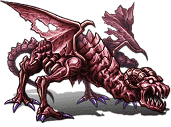
\includegraphics[width=0.28\textwidth]{./art/monsters/zombiedragon.png}}
{
 PV: & \hfill 125 & PM: & \hfill 80\\
 FUE: & \hfill 6 & DEF: & \hfill 5 \\
 MAG: & \hfill 0 & RES: & \hfill 3 \\
 AGI: & \hfill 2 & Tamaño: & \hfill G\\
}
{
 \textbf{Mordida}: 3d de daño, 2u Alcance \hfill \textbf{Botín:} 900 Gil \\
 \textbf{Inmune}:\ko\poison\sleep\silence \hfill \textbf{Débil}:\holy 
 
 \mtech{Aliento Venenoso}{10}{1t}{3u (frente)}{Tú}{Todos los que se encuentren en el área de efecto reciben 4d de daño y hacen una tirada con DC~8. Si fallan, quedan \hyperlink{status}{Envenenados} por 3 turnos.}{\poison} \mreaction{Regenerar}{
 Cuando tus PV sean menos de 50, no puedes moverte ni hacer acción alguna. Regeneras 50 PV en cada turno durante 3 turnos tras los cuales puedes volver a actuar y a moverte. Este efecto solo se puede utilizar una vez por batalla. } \mpassive{No Muerto}{Sufres permanentemente el estado \hyperlink{status}{Zombi}.}
	%\vspace{0.1cm} \hrule \vspace{0.1cm} 
 %\emph{"¡No me comas! ¡No tengo buen sabor!" -- Eiko}
}
